\section{File reading partitioning}

\begin{frame}
 \begin{itemize}
  \item Problem: I have multiple input files and I want to process them in parallel
  \item Solution: use partitioning to parallelize the processing on multiple threads
 \end{itemize}
\end{frame}

\begin{frame}
 \frametitle{Serial processing}
 \begin{center}
 \includegraphics[width=10cm]{figures/input-files-serial.pdf}
 \end{center}
\end{frame}


\begin{frame}
 \frametitle{Partitioning in Spring Batch}
 \begin{itemize}
  \item Partition the input data
  \begin{itemize}
    \item e.g. one input file = one partition
    \item partition processed in a dedicated step execution
  \end{itemize}
  \item Partitioning is easy to set up but need some knowledge about the data
  \item Partition handler implementation
  \begin{itemize}
   \item Multi-threaded
   \item Spring Integration  
  \end{itemize}
 \end{itemize}
\end{frame}

\begin{frame}
 \frametitle{Multi-threaded partitioning}
 \begin{center}
  \includegraphics[width=10cm]{figures/input-files-partitioning.pdf}  
 \end{center}
\end{frame}

\begin{frame}[fragile]
\frametitle{Partitioner for input files}
\begin{xmlcode}
<bean id="partitioner"
      class="o.s.b.core.partition.support.MultiResourcePartitioner">
  <property name="resources" 
            value="file:./src/main/resources/input/*.txt" />
</bean>
\end{xmlcode}
\end{frame}

\begin{frame}[fragile]
\frametitle{The partitioner sets a context for the components}

\begin{xmlcode}
<bean id="reader" 
      class="org.springframework.batch.item.file.FlatFileItemReader" 
      scope="step">
  (...)
  <property name="resource" 
            value="#{stepExecutionContext['fileName']}" />
</bean>
\end{xmlcode}
\end{frame}

\begin{frame}[fragile]
 \frametitle{Using the multi-threaded partition handler}
 \begin{xmlcode}
<batch:job id="fileReadingPartitioningJob">
  <batch:step id="partitionedStep" >
    <batch:partition step="readWriteContactsPartitionedStep"
                     partitioner="partitioner">
      <batch:handler task-executor="taskExecutor" />
    </batch:partition>
  </batch:step>
</batch:job>

<batch:step id="readWriteContactsPartitionedStep">
  <batch:tasklet>    
    <batch:chunk reader="reader" writer="writer" 
                 commit-interval="10" />
  </batch:tasklet>	
</batch:step>
 \end{xmlcode}
\end{frame}

\begin{frame}
 \frametitle{Going further...}
 \begin{itemize}
  \item Spring Integration partition handler implementation
  \item Other scaling approaches
  \begin{itemize}
   \item parallel steps, remote chunking, multi-threaded step)
  \end{itemize}  
 \end{itemize}
\end{frame}

